% !TEX root = /home/Documents/thesis/draft/thesis.tex
\documentclass[12pt,twoside]{reedthesis}

\usepackage{graphicx,latexsym}
\usepackage{amssymb,amsthm,amsmath}
\usepackage{longtable,booktabs,setspace}
\usepackage{fancyvrb}
\usepackage[hyphens]{url}
\usepackage{rotating}
\usepackage{listings}
\usepackage{fancyvrb}
\usepackage{tikz}
\usepackage[backend=biber, style=numeric, sorting=ynt]{biblatex}
\addbibresource{thesis.bib}

\newcommand{\vrb}[1]{\Verb!#1!}

\lstset{	% for source code formatting
basicstyle=\small\ttfamily,
columns=flexible,
breaklines=true
}

\title{Simulating Granularity-Change Caching \\ for Realistic Scalable Systems}
\author{Alan R. Jessup}
% The month and year that you submit your FINAL draft TO THE LIBRARY (May or December)
\date{May 2024}
\division{Mathematics and Natural Sciences}
\advisor{Charles McGuffey}
\department{Computer Science}

\setlength{\parskip}{0pt}
\begin{document}

\maketitle
\frontmatter % this stuff will be roman-numbered
\pagestyle{empty}

\tableofcontents

% If your abstract is longer than a page, there may be a formatting issue.
\chapter*{Abstract}

...

\mainmatter
\pagestyle{fancyplain}

\chapter{Introduction}

\section{A crash course in computer caching}

Computer memory is the fundamental component of digital systems that serves as a dynamic repository for data and instructions to be temporarily stored for quick access and retrieval during active processes. The drastically lower latency of memory requests compared to retrieval of data from a hard drive or SSD makes memory crucial to efficient performance of computers.

A computer's memory is divided into a \textit{memory hierarchy}, which arranges various types of computer memory in tiers based on side and access speed, with faster but smaller and more expensive layers of memory at the top of the hierarchy. Near the top of this hierarchy, as an intermediate step between the processor and main memory, are caches.

\begin{figure}[h]
    \centering
    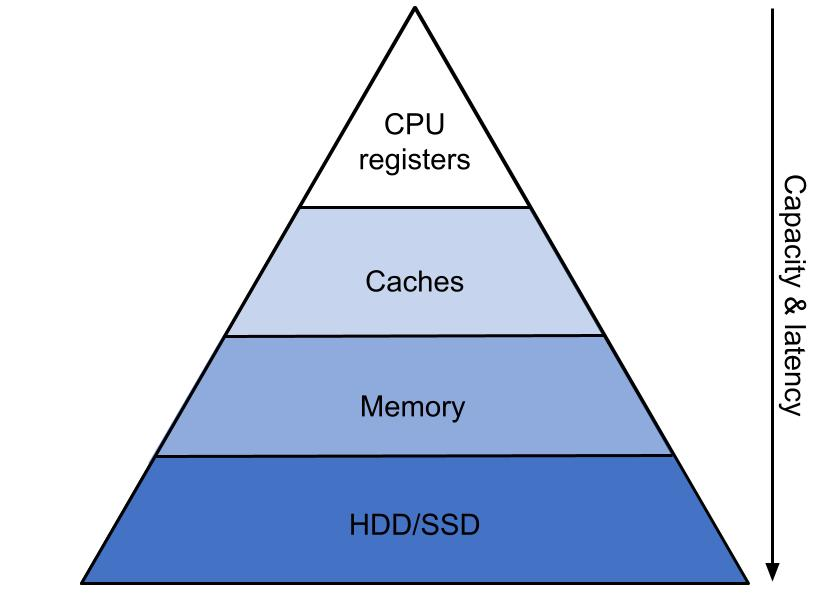
\includegraphics[width=3.5in]{figures/mem_hierarchy.jpg}
    \caption{A diagram of the memory hierarchy.}
\end{figure}

The purpose of caching is to reduce the number of accesses made to the main memory by storing data that is highly likely to be requested in the near future. Since caches are small and fast, intended to be accessed frequently at minimal cost, an important factor of cache design is how to best utilize the limited space they offer. The algorithms that caches use to decide which data to store are called replacement policies, and are typically designed using \textit{spacial} and \textit{temporal locality}.

	\subsection*{Locality}

	Locality is a characteristic of data which caches can use to predict what data is likely to be needed next, in order to store that data and reduce latency.
	
	Data with high temporal locality has been used recently; therefore, it is typically more likely to be needed again than any arbitrary other piece of data. Temporal locality is the more common characteristic used in caching, since it can be as simple to implement as a first-in-first-out (FIFO) queue, and is relatively effective on a wide variety of processes.
	
	Data with spacial locality is data that is located near other data that is being used. This can be useful in specific cases where a large amount of data is stored sequentially, such as frames of a video. Spatial locality is much less well-studied than temporal locality, which the paper Beckmann et. al. aims to improve through introduction of the \textit{granularity-change caching problem}.

	\subsection*{Caches in realistic systems}

	Although upper and lower bounds for cache models can be proven at a theoretical level, realistic estimations of cache performance in complex systems require testing to measure outcomes. The introduction of multiprocessing requires \textit{cache coherence protocols} to maintain consistency across shared memory resources, and multiprocessing adds variable of uncertainty into cache performance, since the structure of a specific processor's cache hierarchy or a particular program's implementation of parallelism can complicate cache behavior.

\section{The granularity-change caching problem}
The 2021 paper ``Spatial Locality and Granularity Change in Caching'' describes and provides a theoretical analysis of the Granularity-Change (GC) Caching Problem, which ``modifies the traditional caching setup by grouping data items into blocks, such that a cache can choose any subset of a block to load for the same cost as loading any individual item in the block'' \cite{beckmann}. This allows a cache to take advantage of both spatial and temporal locality, and creates an opportunity to study tradeoffs of cache space usage between the temporally determined ``item cache'' versus the spatially oriented ``block cache''. For the purpose of implementation, Beckmann et. al. describes the deterministic replacement policy \textit{Item-Block Layer Partitioning}.

	\subsection*{Item-Block Layered Partitioning}

	Item-Block Layered Partitioning (IBLP) is a policy which divides a cache into two virtual segments, one of \textit{item granularity} and the other of \textit{block granularity}.

	\begin{figure}[h]
		\centering
		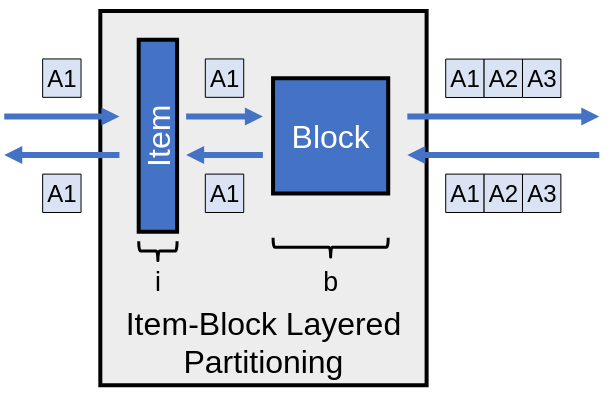
\includegraphics[width=2.5in]{figures/IBLP.png}
		\caption{A diagram of a cache running IBLP \cite{beckmann}.}
	\end{figure}
	
	Beckmann et. al. describes the behavior of IBLP as: \begin{quote}
		The first layer, which serves each access to the cache, loads only the items that are accessed and evicts using the Least-Recently Used (LRU) replacement policy. The second layer, which only serves accesses that miss in the first layer, also uses the LRU policy for evictions, but loads and evicts at the granularity of entire blocks at a time. \cite{beckmann}
	\end{quote}

\section{Prior work simulating GC caching}
In 2022, the Reed College thesis titled ``Simulating the Granularity-Change Caching Problem'', by Maxx Curtis, follows-up the theoretical work of Beckmann et. al. on the granularity-change caching problem by providing a foray into practical simulation of the proposed cache model. Curtis provides a survey of two systems simulators, Zsim and Gem5, and a presents a custom implementation of a block Cache in Gem5 to be used in conjunction with standard Gem5 caches to simulate granularity-change within simple systems \cite{curtis}.

	\subsection*{Results of Curtis}

	The Curtis thesis found 

	\subsection*{Suggestions for future work}

	...

%%%%%%%%%%%%%%%%%%%%%%%%%%%%%%%%%%%%%%%%%%%%%%%%%%%%%%%%%%%%%%%%%
\chapter{Cache Simulation in Gem5}

\section{Background on Gem5 cache models}

	Due to the origins of Gem5 as a combination of two different systems simulation projects, m5 and GEMS, Gem5 contains two separate subsystems that can be used to model caches. The \textit{classic} cache model from m5 provides simple, modular functionality for multi-level caches, but with an inflexible MOESI cache coherence protocol. The \textit{Ruby} cache model has more complex implementation details, with the ability to test customized cache coherence protocols.

	My first approach to simulate IBLP was to follow the method suggested by the Curtis thesis: ``by creating a system with two caches, one for each layer, that differ in granularity and experience little to no intermediate latency'' \cite{curtis}.

\section{Initial classic cache implementation}

	I began by implementing a nestled cache structure using classic Gem5 caches.

	\subsection*{System class}
	For the purpose of organizing and modularizing the facets of the Gem5 system configuration that don't need to be modified for IBLP, I implemented the system setup in a new class, \vrb{StreamlinedSystem}, which inherits the Gem5 \vrb{System} class and adds methods which takes care of setting up the components of a typical system for simulation and piecing together the components of the IBLP cache. [See appendix \#?]

	\subsection*{Cache objects}

	...

	\subsection*{Granularity scope}

	...

\section{Ruby modeling investigation}

	Since the classic cache model failed to meet the requirements for simulating an IBLP cache, I turned to the Ruby cache, to see if the more detailed model had a way of overriding the system-wide line size requirement for a similar implementation using stacked or nestled caches.

	\subsection*{...}

	...

%%%%%%%%%%%%%%%%%%%%%%%%%%%%%%%%%%%%%%%%%%%%%%%%%%%%%%%%%%%%%%%%%

\chapter{Next section}

\section{Something or other}

%%%%%%%%%%%%%%%%%%%%%%%%%%%%%%%%%%%%%%%%%%%%%%%%%%%%%%%%%%%%%%%%%
\chapter{Conclusion}

\section{Results}

...

\section{Future work}

...

%%%%%%%%%%%%%%%%%%%%%%%%%%%%%%%%%%%%%%%%%%%%%%%%%%%%%%%%%%%%%%%%%
\appendix
\chapter{Glossary}

\def\arraystretch{1.5}
\begin{tabular}{p{1.5in}p{3.8in}}
    \hline
    \textbf{Term}       & \textbf{Definition} \\
    \hline
	Block               & In the context of general caching, a standard amount of data. \\
	Block (GC-cache)	& In granularity-change caching, \textit{block} specifically refers to the lower-granularity line size. \\
	Cache coherence		& ... \\
	Granularity         & The size of a data \textit{block}, i.e. cache \textit{line}. A higher granularity has a larger block size, and lower vice versa. \\
	Hit/miss rate 		& ... \\
    Item (GC-cache)  	& In GC-caching, \textit{item} refers to the higher-granularity line size. \\
    Line                & A portion of a cache that contains one \textit{block} of data. \\
	Memory hierarchy	& ... \\
\end{tabular}

%%%%%%%%%%%%%%%%%%%%%%%%%%%%%%%%%%%%%%%%%%%%%%%%%%%%%%%%%%%%%%%%%
\chapter{Source Code and Documentation}

\section{Simulation config}

\subsection*{Caches}
%\lstinputlisting{code/msi_caches.py}
\;\\

\subsection*{Runfile (Config)}
%\lstinputlisting{code/simple_ruby.py}
\;\\

\section{Test scripts}

...

\backmatter % backmatter makes the index and bibliography appear properly in the t.o.c...

\nocite{*}
\addcontentsline{toc}{chapter}{References}
\printbibliography[title=References]

\end{document}
